\usepackage{acronym}\chapter{Introduction}\label{ch:introduction}

\setlength\epigraphwidth{.738\textwidth}
\epigraph{\itshape Life Before Death. Strength Before Weakness. Journey Before Destination.}{Brandon Sanderson, \textit{The Way of Kings.}}

\lettrine{\textcolor{accent_color}{W}}{ho} has never dreamt of a robot friend?
A robot that can help you with your daily tasks, play games with you, help you with your homework, or even be your personal assistant?
The idea of having a robotic companion is not new, for it has remained a dream for humanity for a long time.
Since the first mention of the term \textit{robot}~\cite{robot1920}, this aspiration has been only possible in science fiction movies and books.
However, with the recent advancements in robotics and artificial intelligence, we are closer than ever to this reality.
This humble thesis is nothing more than just a small step towards the joint effort of achieving this dream.

Now, how do we create a robot that can be a friend to humans?
This simple question omits a multitude of challenges that need to be addressed.
Some of these challenges include the robot's ability to understand and interact with humans, its ability to learn from its environment, or its ability to adapt to different situations.
However, there is one aspect underlying all these challenges; \textit{movement}:

\begin{itemize}
    \item A robot that understands and interacts with humans \textit{must be able to move} in order to follow the humans and interact with them.
    \item A robot that learns from its environment \textit{must be able to move} in order to explore and gather information.
    \item A robot that adapts to different situations \textit{must be able to move} in order to change its behavior and actions based on the environment.
\end{itemize}

Moreover, it has been thoroughly discussed in the literature that movement is a fundamental aspect of intelligence~\cite{Darwin1871, Arbib2005, Leisman2016, Wolpert2011, Llinas2001}.
This clearly shows that movement is a crucial component of any intelligent system known to us.
If we want to create any intelligent entity that somehow resembles our own intelligence, we must first address the problem of movement.

This thesis is dedicated to the study of movement in robots, specifically in the context of embodied artificial intelligence.
This topic is known as \acrfull{vsn}, in which and agent must navigate in an environment to accomplish certain tasks while only relying on visual information.
On \acrshort{vsn} there is no prior knowledge of the environment or any map that the agent can consult.
The agent must learn to navigate in the environment by exploring it and learning from its own experiences.
It has to understand the scene not only geometrically, but also semantically.
If not, it will not be able to understand the meaning of the objects in the scene and how they relate to each other.
For example, if the agent is placed in a bedroom and asked to find a fridge, it must understand that the fridge is not (typically) in the bedroom and that it must navigate to the kitchen to find it.

\acrshort{vsn} tasks are very challenging, and as one may expect, they typically need a careful design of a complex system that combines multiple components in charge of different aspects of the navigation.
Many works~\cite{newcombe2011, thrun2001, jones2011, sattler2018, Kazerouni2022, campos2021, labbe2022, zhang2018, rosinol2020, jin2023} follow this approach, and they typically rely on a combination of visual perception, semantic understanding, and navigation planning.
However, \acrshort{vsn} can be also formulated as a \acrfull{rl}~\cite{sutton2018} problem.
\acrshort{rl} is a whole artificial intelligent framework that allows an agent to learn how to act in an environment by receiving rewards for its actions.
The rewards are typically defined in terms of the agent's performance in the task, such as reaching a goal or avoiding obstacles.
By following an iterative process within the environment, the agent can learn how to maximize its rewards and complete its tasks.

The main goal of this thesis is to study the \acrshort{rl} and \acrshort{vsn} powerful combination that allows agents to be trained to navigate in an environment.
After intensive training, agents can learn to navigate by trial and error, obtaining rewards that guide them to the goal.
In figure~\ref{fig:abstract_thesis}, an abstract representation of the thesis's framework is shown.
In it, an agent, by interacting with the environment, learns to navigate to a goal.
In the environment, even though there is not a map present, the agent can learn to understand the scene and the objects in it.
By these semantic cues, the agent can learn to navigate to the goal, even if it is not visible in the scene.

\begin{figure}
    \centering
    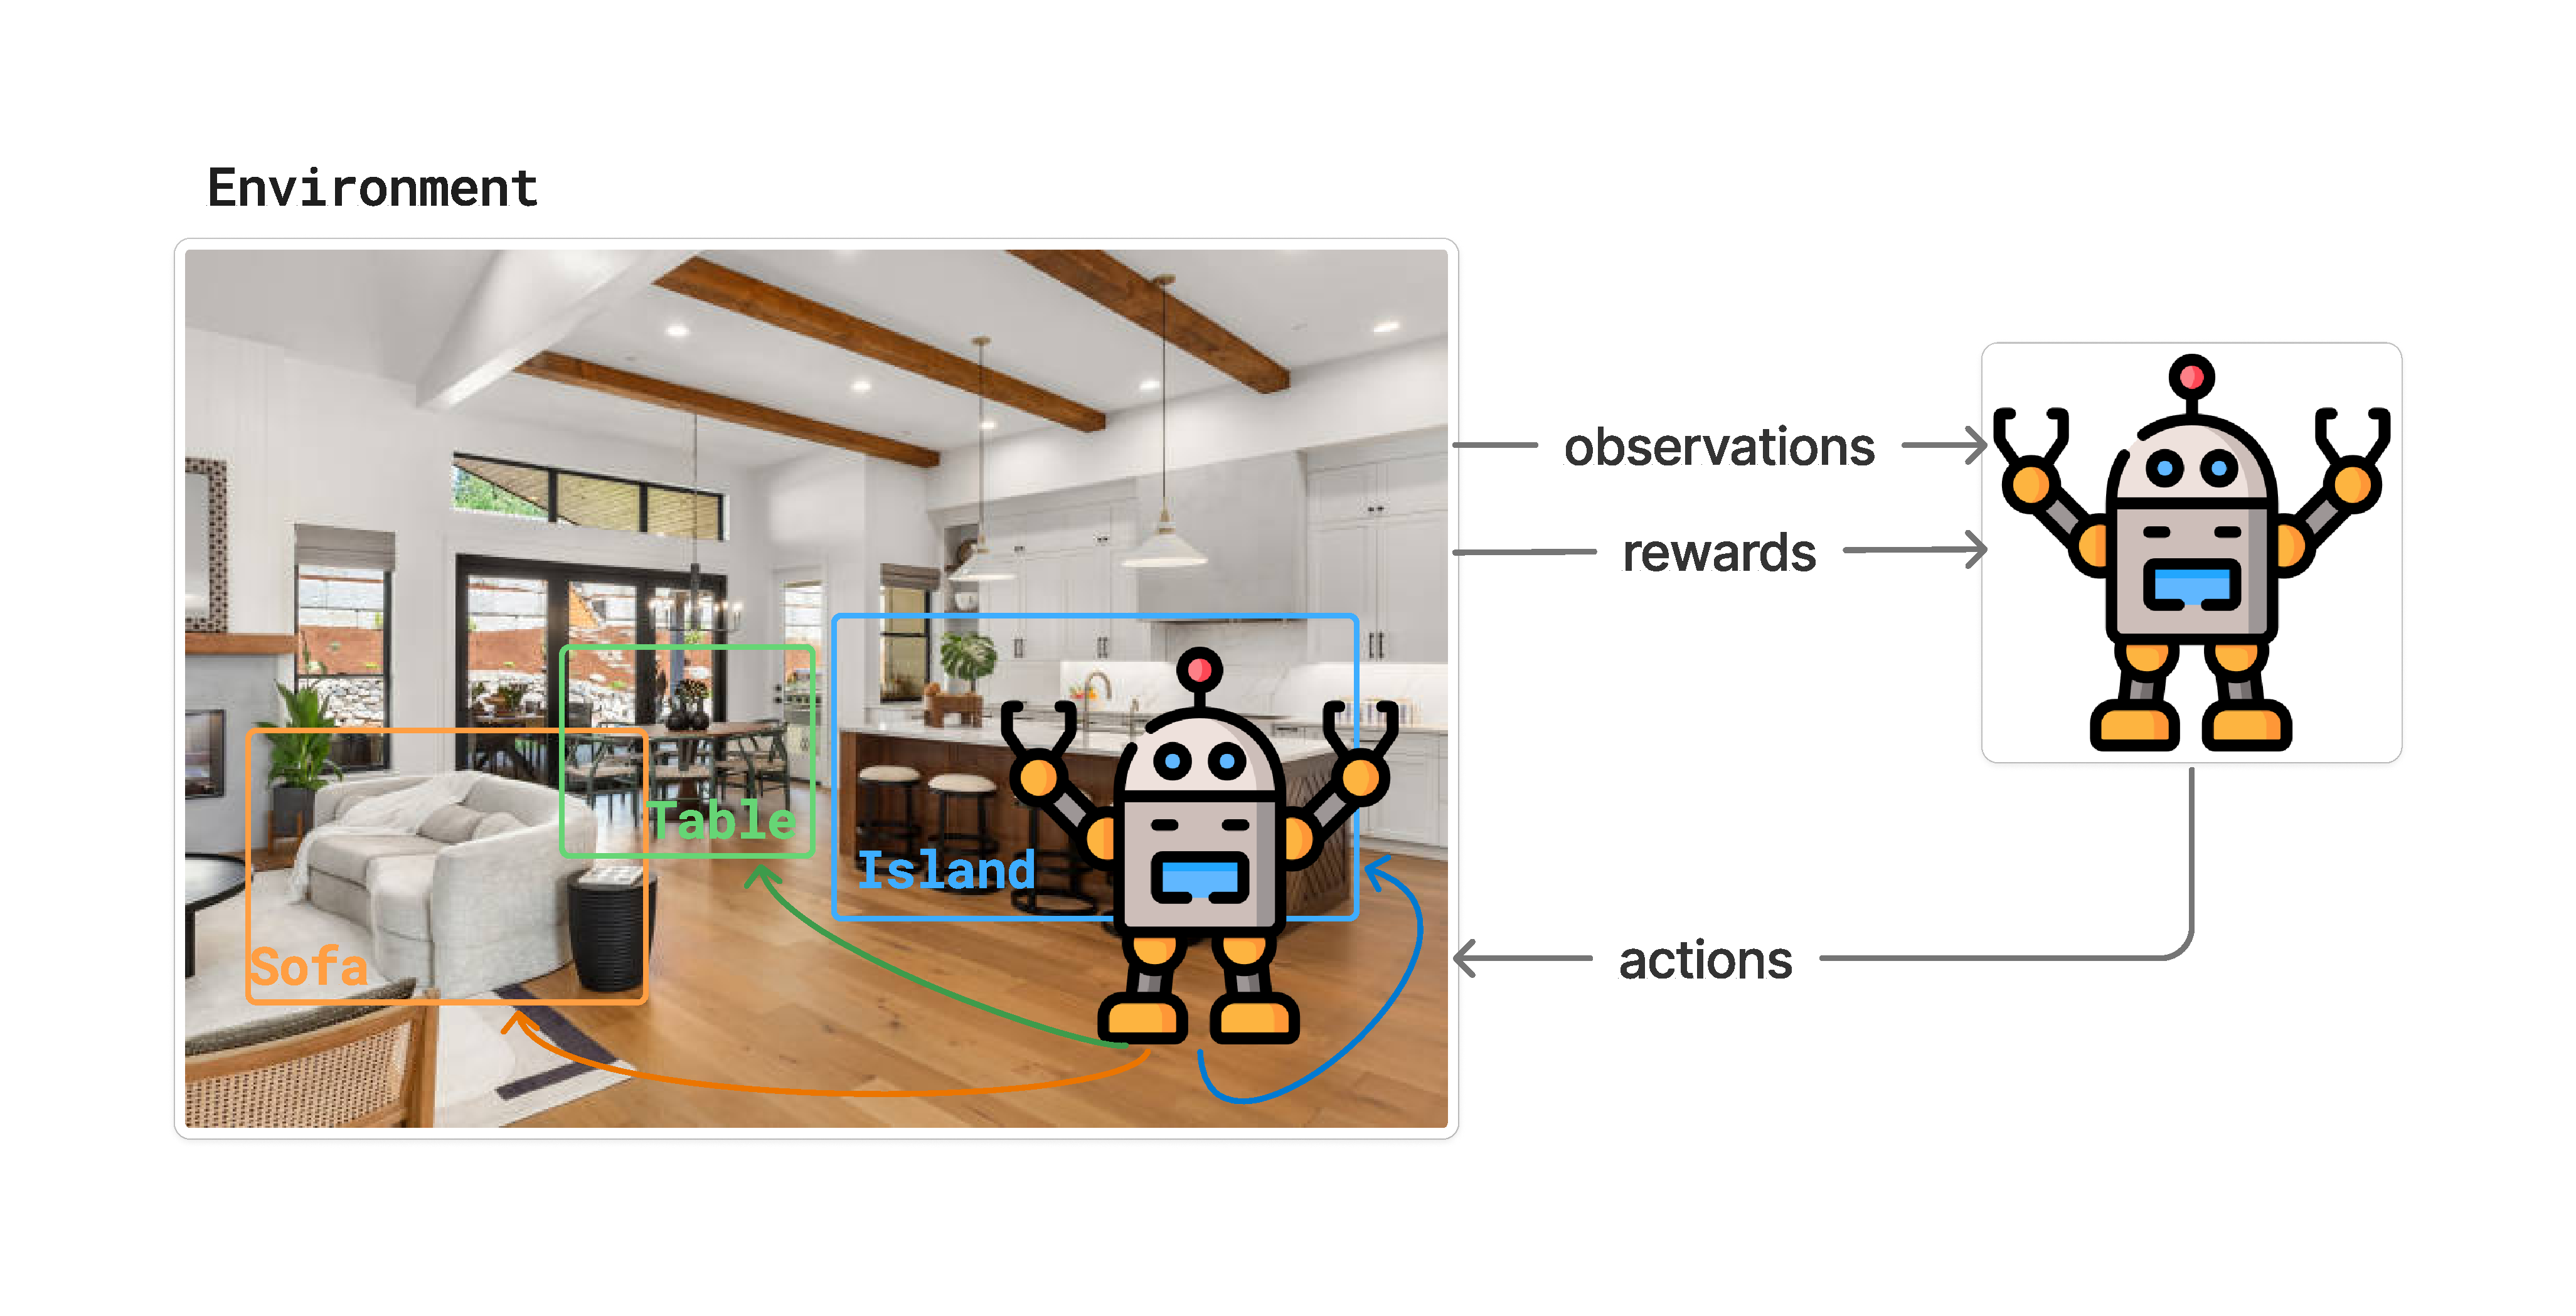
\includegraphics[trim=30 30 30 30, clip, width=\textwidth]{figures/introduction/abstract_thesis}
    \caption{\textbf{The framework of \acrshort{rl} and \acrshort{vsn}}. Navigating in an environment is a complex task that requires the agent to learn how to interact with the environment and understand the scene. The agent learns to navigate by trial and error, obtaining rewards that guide it to the goal. In this way, the agent can learn to understand the scene and the objects in it, even if there is no prior knowledge of the environment or any map that it can consult.}
    \label{fig:abstract_thesis}
\end{figure}

\section{Motivation}\label{sec:motivation}

This thesis is part of the AIRPLANE (Artificial Intelligence and Robotic Mobile PLAtforms to Improve Disabled People INdependencE) research project conducted in the~\href{https://gramweb.uah.es/}{GRAM research group} of the~\href{https://www.uah.es/en/}{University of Alcalá}.
The AIRPLANE project focuses primarily on creating new mobile robotic platforms that incorporate advanced perception, interaction, and navigation capabilities to enhance the independence of people with functional diversity.
The main goal in the AIRPLANE project is to build a low-cost mobile platform that integrates the latest advances in artificial intelligence and computer vision.
Specifically, it will equip the platform with the ability to navigate real environments and develop online action-recognition solutions that enable interaction applications for users with functional diversity.
And, as shown in the figure~\ref{fig:icra_papers}, the interest in this topic is not only limited to the AIRPLANE project, but it is also a hot topic in the robotics community.
Therefore, the first step is to study \acrshort{vsn} solutions that allow the robot to navigate using \acrshort{rl} algorithms.

The \acrshort{vsn} problem is very broad, and it can be applied to many different scenarios.
For example, it can be used to navigate in indoor environments, such as homes or offices, or in outdoor environments, such as streets or parks.
It can be used to navigate in environments with different types of obstacles, such as furniture or people, or in environments with different types of goals, such as finding a specific object or reaching a specific location.
It can also be used to perform different types of tasks, such as rearranging objects~\cite{NEURIPS2021_021bbc7e}, navigating to them~\cite{batra2020}, or even performing a natural language description of the scene~\cite{Tan2021EmbodiedSD}.
In this thesis, the main focus will be on navigating in indoor environments, specifically reaching certain object goals.

Since the first time \acrshort{rl} was applied to navigation~\cite{MAHADEVAN1992311}, many works have been proposed to tackle this problem.
However, the vast majority of them rely on simulated environments, such as the \textit{ProcTHOR}~\cite{Deitke2022ProcTHORLE} or \textit{Habitat}~\cite{NEURIPS2021_021bbc7e} platforms.
These platforms are invaluable for training agents in a controlled environment, because they can provide a massive scale of training data and allow for fast iterations that can lead to the emergence of complex behaviors~\cite{Wijmans2022EmergenceOI}.
Despite the advantages of these platforms, deploying algorihtms trained on simulation on real-world scenarios can be very challenging.
Several problems can arise, such as the \textit{sim-to-real} gap~\cite{kadian2020}, or the domain shift~\cite{kim2022}.
This document focuses on the study of \acrshort{vsn} in real-world scenarios, and how to overcome the challenges that appear when trying to deploy simulation-trained models on the real world.

\begin{figure}
    \centering
    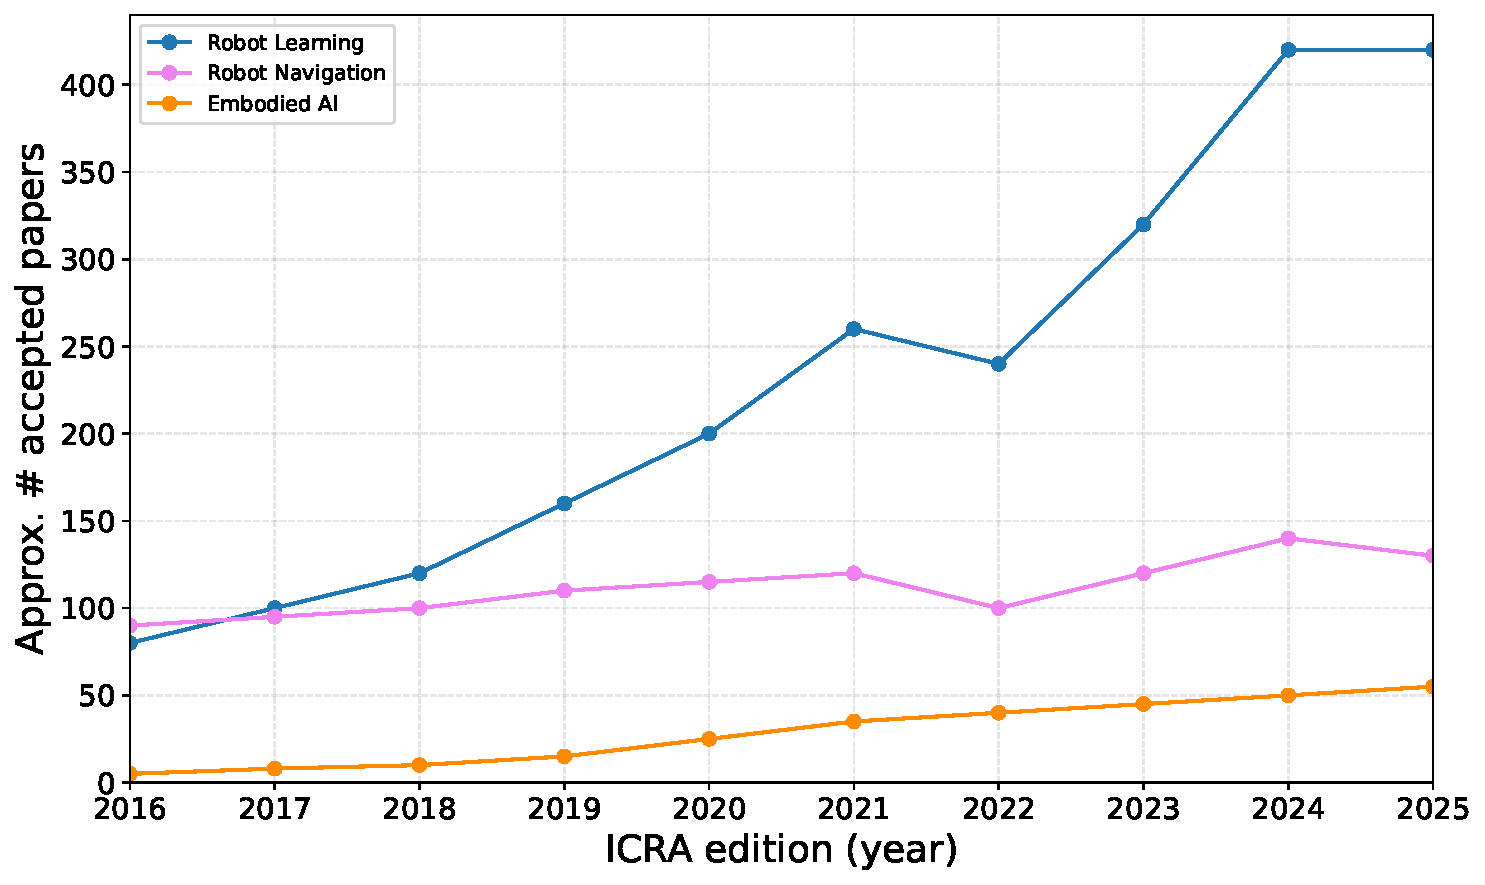
\includegraphics[width=\textwidth]{figures/introduction/icra_papers}
    \caption{\textbf{Robot learning, navigation, and embodied AI accepted papers on IEEE International Conference on Robotics and Automation (ICRA) over the last ten years}. The number of accepeted papers is calculated by rule-based grep over the abstracts of the accepted papers in the ICRA proceedings. They show how typical topics in robotics that study \acrshort{vsn} have been gaining popularity over the years.}
    \label{fig:icra_papers}
\end{figure}

Beyond the research project that motivates this thesis, the ultimate goal of this thesis is to provide with a comprehensive study of \acrshort{vsn} and \acrshort{rl} algorithms that can be helpful for many applications.
Some of these applications, but not all, include:
\begin{itemize}
    \item \textbf{Assistive robots}: Robots that can help people with functional diversity to navigate in their environment and perform daily tasks.
    These robots need to be able to develop enough intelligent behaviors to understand the environment and the people in it, and to adapt to their needs.
    \item \textbf{Hazardous environments}: Robots that can navigate in environments that are dangerous for humans, such as disaster areas or nuclear plants.
    They can circumvent obstacles, find victims, or even perform tasks that are too dangerous for humans.
    This is a powerful application of \acrshort{vsn} that can save lives and reduce risks for humans.
    \item \textbf{Vertical-farm inspection robots}: Robots that can navigate densely packed hydroponic racks, visually distinguish crop maturity or disease markers, and localize specific trays for targeted harvesting or treatment.
    \item \textbf{Planetary or subterranean exploration rovers:} build semantic maps of unseen caves, lava tubes, or Martian terrain, finding scientific targets while avoiding hazardous slopes without GPS.
    \item \textbf{Immersive VR/AR game characters:} NPCs use the same visual scene the player sees (no cheat-sheet nav meshes) so they naturally avoid furniture, peek around corners, and respond to spoken commands (“guard the green door”).
\end{itemize}

\section{Contributions of the Thesis}\label{sec:contributions-of-the-thesis}

The main contributions of this thesis are summarized as follows:
\begin{itemize}
    \item A comprehensive study of the literature of the \acrshort{vsn} setting and a thorough study of the \acrshort{rl} algorithms that can be applied to real-world scenarios.
    This includes a review of the state-of-the-art methods, their limitations, and the challenges that need to be addressed.
    Thanks to this, the ready can understand the current state of the art in \acrshort{vsn} and \acrshort{rl}, and contextualize the main goals of this document.
    \item A clear definition of the \acrshort{vsn} problem, and a set of benchmarks that can be used to evaluate the performance of \acrshort{vsn} algorithms in simulated environments.
    It also includes a set of metrics that can be used to evaluate the performance of different techniques such as $\epsilon$-greedy exploration or different reward functions.
    \item A comprehensive study of the different \acrshort{vsn} algorihtms in real-world scenarios.
    This includes a definition of an experimental setup that can be used to evaluate the performance of different models in real-world environments.
    On top of that, this also includes the release of a novel ROS package called ROS4VSN that provides a set of tools and utilities to facilitate the development of \acrshort{vsn} algorithms in real-world scenarios.
    \item A novel approach to \acrshort{rl} that combines the advantages of Offline Reinforcement Learning~\cite{levine2020} with DD-PPO~\cite{Wijmans2019DDPPOLN} to train \acrshort{vsn} agents without the need to query any environment, just by using offline data.
    \item
\end{itemize}

\section{Thesis Structure}\label{sec:thesis-structure}

The structure of this thesis is as follows: